\chapter{INTRODUÇÃO}
\label{c.introducao}

A presença das redes de computadores no cotidiano vem aumentando de modo muito
veloz há anos e apresentou um crescimento em especial com o advento das redes
sem fio e da produção massiva e a queda do custo de dispositivos portáteis
capazes de se conectarem à internet. De maneira proporcional, aumentaram-se
também os riscos relacionados à segurança de redes e à privacidade de
informações de diversas espécies que trafegam por entre elas e seus usuários.
Numa proposição inicial, este trabalho define como \textit{Malware} todo tipo de
programa que seja capaz de alterar o comportamento de um software num
dispositivo conectado a uma rede qualquer, feito com o desejo de vender
informações de usuários, causar desordem, roubar credenciais, enviar \textit{spams},
alimentar motores de otimização de busca (SEO) com informações falsas sobre
visitas a páginas da Web ou ainda de chantagear usuários, como foi o caso do
\textit{malware} japonês denominado \textit{Kenzero}, que publicava históricos de navegação
juntamente com a identificação de seus usuários, a menos que os mesmos
pagassem 1500 ienes para que seus dados fossem retirados do acesso ao público.
SAWLE et al. (\citeyear{sawle14}).

De acordo com IDIKA (\citeyear{idika07}), pode-se classificar os tipos de
métodos de detecção de maneira mais rudimentar em duas categorias: detecção
baseada em anomalia e detecção baseada em assinatura. A detecção por anomalia
é uma técnica que consiste em treinar um algoritmo de detecção para que ele
“saiba” o que constitui o comportamento normal de um programa, para que ele
possa decidir sobre a periculosidade dos programas a serem inspecionados. Essa
mesma abordagem também dá origem a uma técnica muito similar conhecida como
detecção baseada em especificações, onde levantam-se especificações e
conjuntos de regras para que a partir daí defina-se o comportamento de um
programa normal. A técnica de detecção por assinaturas, por sua vez, envolve a
caracterização do que já seria sabidamente malicioso para encontrar traços
semelhantes e encontrar os programas anômalos. Todas as técnicas citadas acima
podem ser aplicadas com um de três modos diferentes, sendo eles análise
estática, análise dinâmica e análise híbrida, onde a análise estática num
contexto de detecção por assinaturas, verificaria aspectos estruturais de
programas inspecionados, como sequências de \textit{bytes}, e a análise dinâmica
buscaria informações de maneira concorrente ao tempo de execução do programa.
Em suma, a análise estática procura investigar o programa antes que ele seja
executado, e a análise dinâmica atua ou na execução do programa, ou depois que
ele já foi executado. As técnicas híbridas são simplesmente combinações dessas
duas anteriores, juntando informações estáticas e dinâmicas para que se
conclua um parecer sobre a maliciosidade dos códigos analisados.

Dessa maneira, é possível exemplificar as técnicas de detecção com a figura 1:

\begin{figure}[H]
\caption{\small Classificação das técnicas de detecção de \textit{Malware}}
\centering
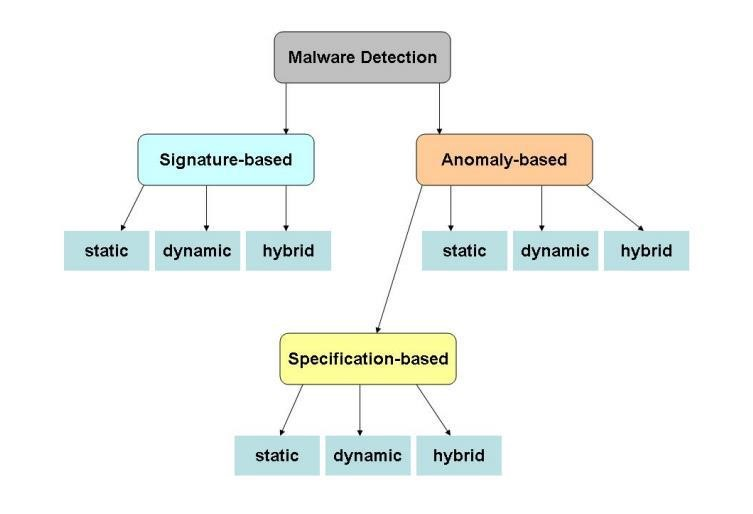
\includegraphics[scale=0.8]{figs/fig1}
\label{f.metodos_deteccao_01}
\legend{\small Fonte: Elaborada pelo autor.}
\end{figure}

Nesta seção do texto, ainda será explicado o problema que o projeto se propõe a resolver, os objetivos esperados para a implementação e a justificativa para o estudo que se desenvolveru no tema. No capítulo 2
encontra-se todo o referencial teórico que permeia os conceitos de redes, segurança de redes, famílias de
\textit{malware} e outros conceitos relacionados ao projeto. No capítulo 3 estão as informações sobre as ferramentas que foram utilizadas na fase de implementação, documentada no capítulo 4. O capítulo 5 conclui o texto com algumas considerações sobre estudos futuros e os resultados obtidos em vários aspectos do projeto.

\section{Problema}
\label{c.problema}

Os dispositivos móveis atuais ainda não possuem capacidade computacional disponível para que se façam varreduras constantes que utilizem as técnicas de
detecção dinâmicas em seus respectivos sistemas à procura de código malicioso,
e com a abrangência da internet se tornando cada vez mais expressiva, o dano
em potencial que um \textit{malware} pode causar a um determinado indivíduo, ou ainda
em grupos massivos também torna-se mais preocupante. Sob a ótica de Szewczyk
(\citeyear{szewczyk12}), as redes de computadores, principalmente sem fio, começam a apresentar
problemas de vulnerabilidade a partir do momento da compra do \textit{hardware}
necessário para implementação da rede e da configuração desse equipamento,
onde muitas vezes os vendedores destes produtos tentam passar a ideia de que
os equipamentos por si são capazes de blindar uma rede contra qualquer
intrusão, a fim de obter sucesso comercial valendo-se da ingenuidade de
usuários leigos no assunto de segurança de redes. As técnicas de detecção por
assinatura, apesar de não serem as mais eficazes à disposição, são muito mais
simples de se implementar e resolverem o problema da infecção por \textit{malwares}
conhecidos ou ainda \textit{malwares} novos com características semelhantes às dos
conhecidos.

\section{Objetivos e justificativa}
\label{s.objetivos}

\subsection{Objetivo Geral}
\label{s.objetivog}

Analisar o resultado da ação de diferentes técnicas de detecção de \textit{malware}
baseadas em assinatura num ambiente de testes para obter métricas relevantes
quanto à eficiência nas varreduras realizadas, número de falsos positivos
encontrados e se possível determinar qual delas é a mais apropriada para uso
em ambientes \textit{mobile} e de redes de computadores em geral.
 
\subsection{Objetivos Específicos}
\label{s.ojetivosp}

- Para embasar o projeto, foi levantado um histórico sobre segurança em redes
  de computadores e assuntos correlacionados principalmente às técnicas de
  detecção a serem estudadas.

- Montar um ambiente para que ele seja populado com conjuntos de programas a
  serem investigados e executar diferentes algoritmos para que posteriormente
  classifiquem-se seus resultados. Por questões de relevância, o escopo do
  trabalho envolverá sistemas \textit{Windows} e \textit{Android} pois a maioria dos usuários
  comuns utiliza estes sistemas operacionais.

- Comparar todos os métodos previamente escolhidos e testados para apresentar
  suas respectivas características e desempenhos.


\subsection{Justificativa}
\label{s.justificativa}

O desenvolvimento de novas técnicas de segurança computacional, bem como a
análise e aprimoramento de técnicas já construídas anteriormente, representam
sempre um avanço na área de segurança de redes, pois todo tipo de sistema
operacional possui alguma deficiência no quesito de segurança, haja visto que
mesmo agências de inteligência como a NSA enfrentam de tempos em tempos
problemas envolvendo vazamentos de dados e intrusões. De acordo com HASSAN (\citeyear{hassan10}), os tipos de ataque mais poderosos e bem
sucedidos ocorrem de dentro da rede, pois em diversas situações, o
administrador de rede confia em todos os usuários internos e não suspeita de
ataques vindos de seu próprio lado. Por isso, é sempre um investimento
desenvolver e manter uma política de aprimorar as defesas das redes de
computadores. O contexto do projeto é o da esfera do usuário comum, que
utiliza dispositivos comuns mas também é alvo de ataques que às vezes são
menores e até inofensivos, que contudo, ocorrem com frequência.